\section{System Overview}
\begin{figure}
\centering
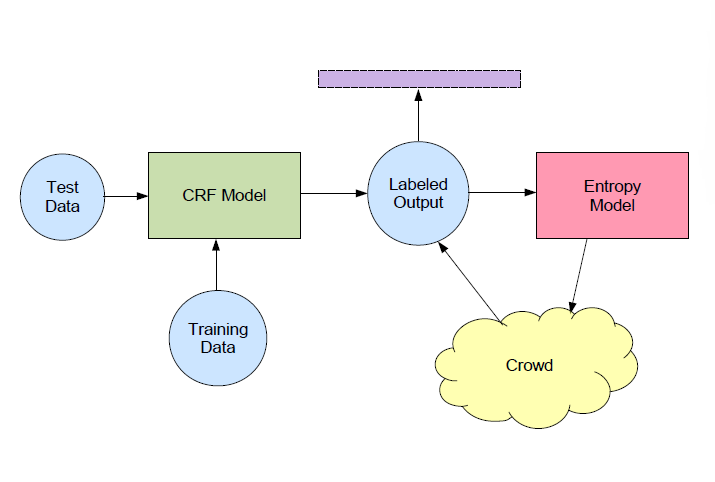
\includegraphics[width=0.5\linewidth]{images/system_design.png}
\label{fig:system_design}
\caption[example]{The CrowdPillar system design.  The top uncertain labeled outputs as determined by the entropy model are sent to the crowd.  The purple box denotes the specified application where the labeled data is ultimately sent.}
\end{figure}

The CrowdPillar system design is shown in \ref{fig:system_design}. The core of the system is designed as a modification to probabilistic databases that utilize PGMs as their data model.  Crowdpillar analyzes the uncertainty in the output and generates questions for crowd submission to reduce a Total Utility Function (TUF).  This is discussed in greater detail in Section 4.  The response of the crowd is combined in a principled way with the original PGM output using Dempter-Shafer belief theory, as described in Section 5.

In this paper we consider a sample application task and follow it through the major components of the system: the probabilistic database, question formulation, crowd submission, and data fusion.

Consider an extraction system for automatically reading published citations and storing them in the database.  In order to fit an incoming citation into any nontrivial schema, the string has to be appropriately chunked to determine which tokens belong to which attributes.  A string such as:
\begin{quotation}
\textit{Perfect Model Checking via Unfold/Fold Transformations. Maurizio Proietti, Alberto Pettorossi CL 3-540-67797-6 Springer Lecture Notes in Computer Science Computational Logic - CL 2000, First International Conference, London, UK, 24-28 July, 2000, Proceedings 2000}
\end{quotation}
needs to be labeled with its appropriate title, author, conference, etc.  This is in general a nontrivial problem, especially when one considers the numerous styles and orderings different citations come in.  An efficient extraction system must be trained to handle these different occurences.

The state of the art model for this type of information extraction task is the conditional random field.  We focus specifically on CRFs for the remainder of the paper and make it the flagship example of CrowdPillar, though there exist other models that can derive the appropriate labelings and confidences for which CrowdPillar would also apply.  After the CRF has segmented and labeled the data, each label sequence is stored as a possible world as in Figure (\ref{fig:CRFexample}b)

The goal of CrowdPillar is to optimally select a number of sequences of high uncertainty from the CRF output and query the crowd for the label of each token in a sequence with the highest individually assigned score.  We discuss specifically how scoring is done in Section 4 and how many questions can be asked depends on the user's cost and time budget.  An on-line approach to selecting sequences is highly inefficient due to the relatively slow speed of returning a crowd response (on the order of hours) as well as the high parallelizability of largely independent sequences.  For these reasons, sequences are selected in a batch for submission to the crowd.

After determining which sequences should be sent, we generate a question in XML format for each sequence.  Questions may be in the form of multiple choice, fill in the label, yes/no, etc.  Given the possible uncertainty in the crowd response, we resolve conflict and combine multiple answers to each question using Dempster-Shafer belief theory based on a quality metric attached to each answer to ultimately generate a probabilistic collection of responses to each question.  The quality $Q\rightarrow[0,1]$ may take a number of different forms, including difficulty of the question and approval rating and bias of the responder.  It represents the confidence we have in the answer being correct as opposed to being a randomly generated guess.

The crowd submissions are sent back to the PDB upon completion, where they are combined with the original output CRF data using the Dempster-Shafer Theory of Evidence.  The answers can be returned at once upon completion of the batch or queried in intervals.  How often to specifically query for answers will be dependent on the user's specifications and needs. 

